\section{Příklad 2}
% Jako parametr zadejte skupinu (A-H)
\druhyZadani{G}
\subsection{Výpočet Re}
\begin{figure}[H]
    \centering
    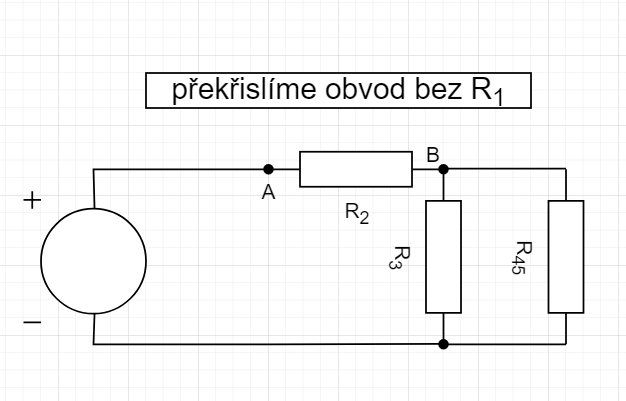
\includegraphics[scale=0.5]{picturesFor2Uloha/1.png}
    \caption{Seriove zapojeni $R_4 \: a \: R_5$}
    \label{fig:Serial_resistor_R45}
    \begin{quote}
    \centering
    $R_{45} = R_4 + R_5$ \\~\\
    $R_{45} = 180\Omega + 460\Omega = 640\Omega$
    \end{quote}
\end{figure}

\begin{figure}[H]
    \centering
    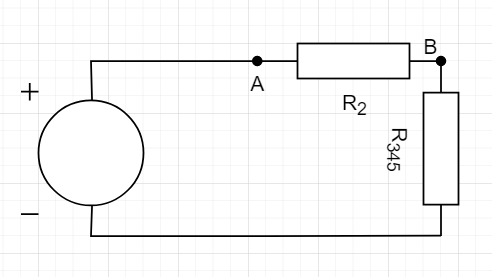
\includegraphics[scale=0.5]{picturesFor2Uloha/2.png}
    \caption{Paralelne zapojeni $R_{45} \: a \: R_3$}
    \label{fig:Paralel_resistor_R345}
    \begin{quote}
    \centering
    $R_{345} = \dfrac{R_{45} * R_3}{R_{45} + R_3}$ \\~\\~\\
    $R_{345} = \dfrac{640\Omega * 615\Omega}{640\Omega + 615\Omega} = \dfrac{393 600\Omega}{1255\Omega} = 313.6254\Omega$
    \end{quote}
\end{figure}

\begin{figure}[H]
    \centering
    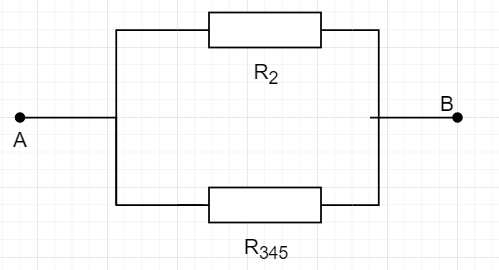
\includegraphics[scale=0.5]{picturesFor2Uloha/3.png}
    \caption{Paralelne zapojeni $R_{345} \: a \: R_2$}
    \label{fig:Paralel_resistor_R2345}
    \begin{quote}
    \centering
    $R_e = R_{2345} = \dfrac{R_{345} * R_2}{R_{345} + R_2}$ \\~\\~\\
    $R_e = \dfrac{313.6254\Omega * 315\Omega}{313.6254\Omega + 315\Omega} = \dfrac{98792.001\Omega}{628.6254\Omega} = 157.1556\Omega$
    \end{quote}
\end{figure}

\subsection{Výpočet Ue}

\begin{figure}[H]
    \centering
    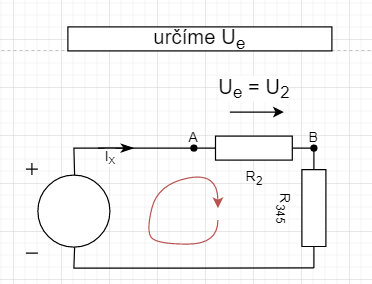
\includegraphics[scale=0.5]{picturesFor2Uloha/4.png}
    \begin{quote}
        \centering
	    Vypočítáme pomocí napětoví děliče \\~\\ 
	    $U_e = U * \dfrac{R_2}{R_2 + R_{345}} $ \\~\\
	    $U_e = 180\Vo * \dfrac{315\Omega}{315\Omega + 313.6254\Omega}  = 
	    180\Vo * \dfrac{315\Omega}{628.6254\Omega} = 90.1968\Vo$ \\~\\
	   
    \end{quote}
\end{figure}
\begin{figure}[H]
    \centering
    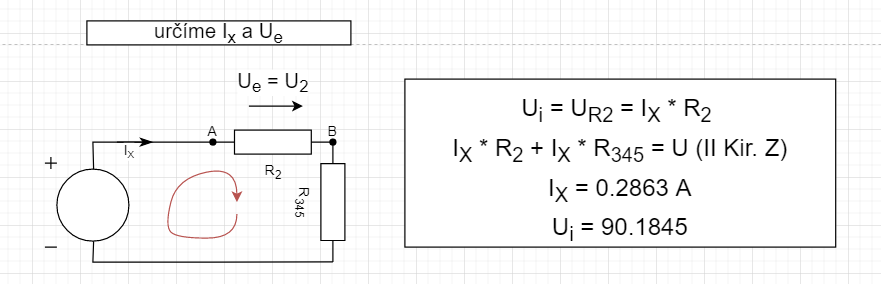
\includegraphics[scale=0.5]{picturesFor2Uloha/4_druhy_zpusob.png}
    \caption{Druhy zpusob reseni}
\end{figure}

\subsection{Výpočet $U_{R1} \: a \: I_{R1}$}

\begin{figure}[H]
    \centering
    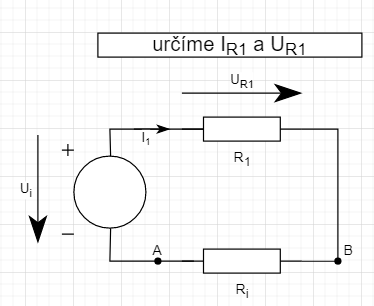
\includegraphics[scale=0.5]{picturesFor2Uloha/5.png}
    \begin{quote}
        \centering
	   $I_{R1} = \dfrac{U_i}{R_1 + R_e} = \dfrac{90.1968\Vo}{250\Omega + 157.1556\Omega}
	   = \dfrac{90.1968\Vo}{407.1556\Omega} = 0.2215290665288651\Am$ \\~\\
	   $U_{R1} = R_1 * I_{R1} = 250\Omega * 0.2215290665288651\Am = 55.3822\Vo$
    \end{quote}
\end{figure}